\subsubsection{UC5 - Generazione \glossario{prompt}}\label{UC5}

\begin{figure}[H]
  \centering
  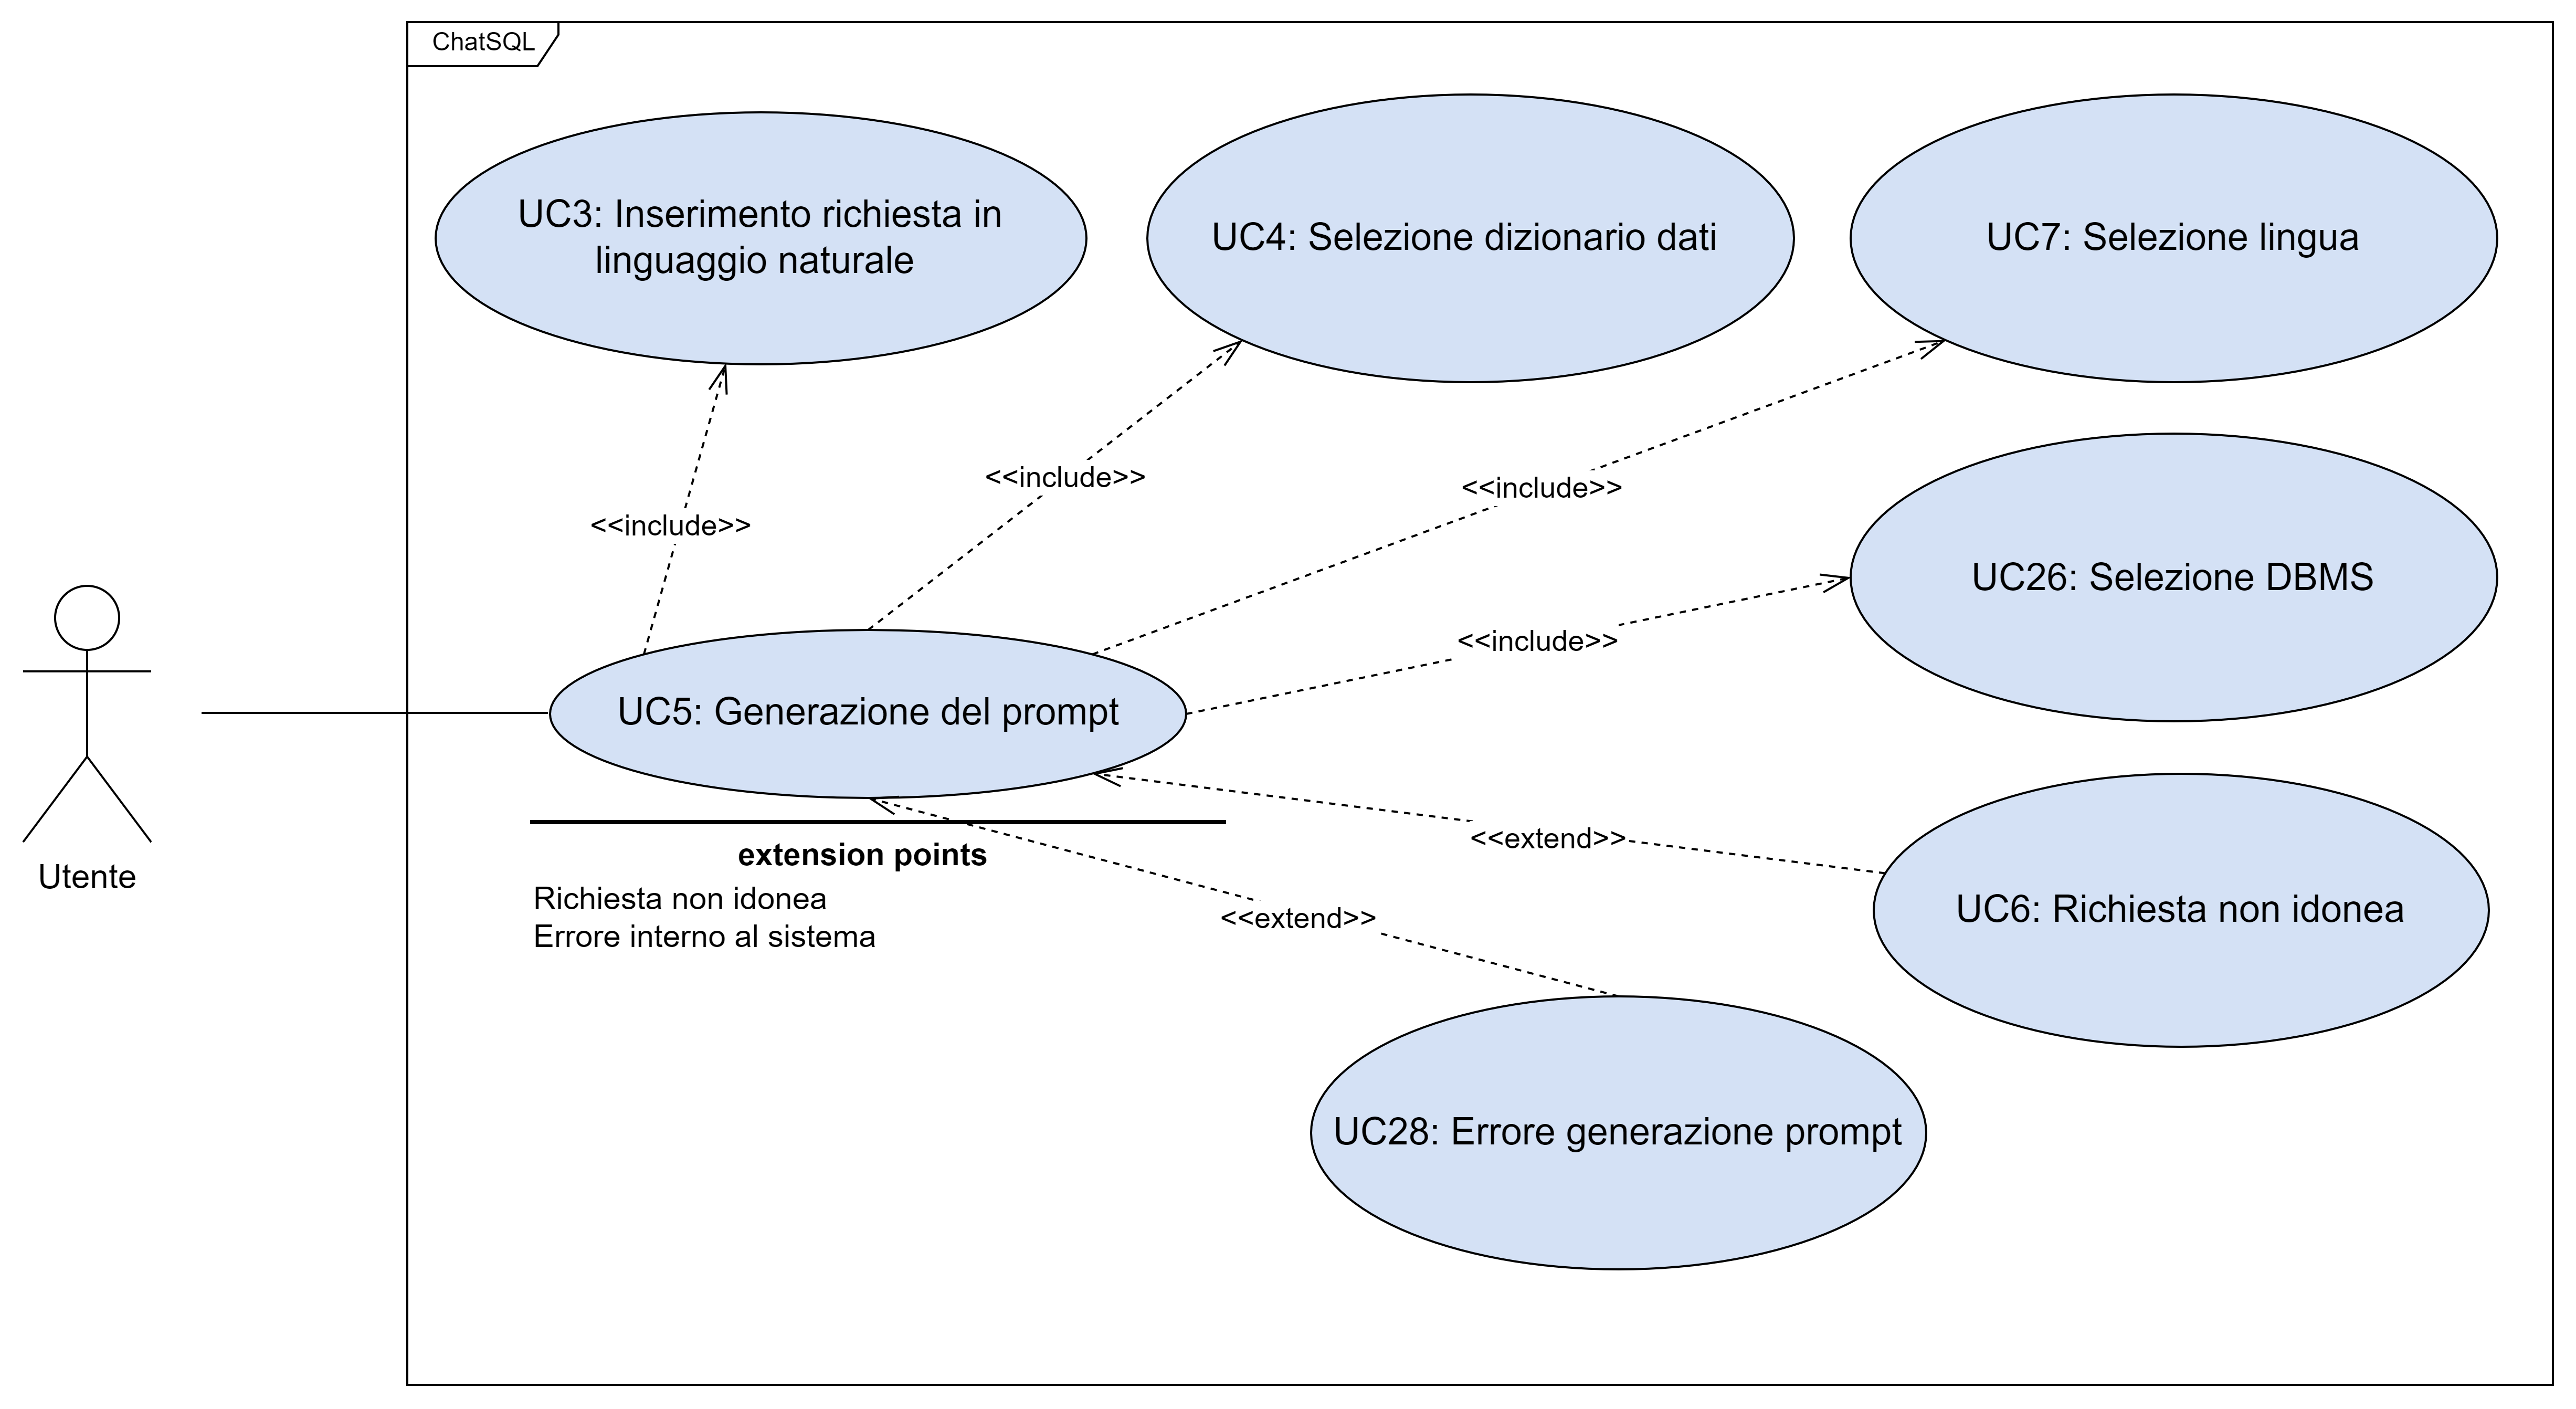
\includegraphics[width=0.90\textwidth]{assets/uc5.png}
  \caption{UC5}
\end{figure}

\paragraph*{Descrizione}
Il sistema genera un \glossario{prompt} a partire da una richiesta dell'Utente in linguaggio naturale, cercando delle corrispondenze con il \glossario{dizionario dati} selezionato.

\paragraph*{Attori principali}
Utente

\paragraph*{Precondizioni}
\begin{itemize}
  \item L'applicazione è stata avviata con successo;
  \item È presente almeno un \glossario{dizionario dati} nel sistema.
  \item L'indice vettoriale (per la ricerca semantica) è stato creato a partire dal \glossario{dizionario dati}.
\end{itemize}

\paragraph*{Postcondizioni}
\begin{itemize}
  \item Il sistema ritorna con successo il \glossario{prompt} corrispondente alla richiesta dell'Utente. Il prompt contiene i \glossario{metadati} estratti dal \glossario{dizionario dati} scelto.
\end{itemize}

\paragraph*{Trigger}
L'Utente desidera ricevere un \glossario{prompt} da fornire in input a un modello di AI esterno al fine di ottenere una \glossario{query} SQL.

\paragraph*{Scenario principale}
\begin{enumerate}
  \item L'Utente seleziona un \glossario{dizionario dati}(\hyperref[UC4]{UC4}), un \glossario{DBMS} (\hyperref[UC26]{UC26}) e una lingua per la richiesta (\hyperref[UC7]{UC7});
  \item L'Utente inserisce un'interrogazione in linguaggio naturale (\hyperref[UC3]{UC3});
  \item Viene avviato il processo di generazione del \glossario{prompt} e di raccolta dei \glossario{metadati} dal \glossario{dizionario dati};
  \item Il sistema restituisce il \glossario{prompt} generato.
\end{enumerate}

\paragraph*{Inclusioni}
\begin{itemize}
  \item Selezione \glossario{dizionario dati} (\hyperref[UC4]{UC4});
  \item Inserimento richiesta in linguaggio naturale (\hyperref[UC3]{UC3});
  \item Selezione lingua (\hyperref[UC7]{UC7});
  \item Selezione DBMS (\hyperref[UC26]{UC26}).
\end{itemize}

\paragraph*{Estensioni}
\begin{itemize}
  \item Richiesta non idonea (\hyperref[UC28]{UC28}).
  \begin{itemize}
    \item Extension point: richiesta non idonea per il modello di AI o per il \glossario{dizionario dati} scelto.
  \end{itemize}
  \item Errore nella generazione del \glossario{prompt} (\hyperref[UC28]{UC28}).
    \begin{itemize}
      \item Extension point: errore interno al sistema.
    \end{itemize}
\end{itemize}